\documentclass[UTF8]{ctexart}
\usepackage[a4paper,margin=1.8cm]{geometry}
\usepackage{graphicx}
\usepackage{float}
\usepackage{longtable}
\usepackage{array}
\usepackage{xcolor}
\usepackage{fancyvrb}
\usepackage{hyperref}
\setlength{\parindent}{0pt}
\setlength{\parskip}{0.45em}
\begin{document}
\section*{最简综合模拟卷}

\subsection*{A 卷题目}

\subsubsection*{一、词法分析：正则表达式、NFA、DFA、最小化（20 分）}

给定正则表达式：

\begin{Verbatim}[fontsize=\small,breaklines=true]
(a|b)*abb
\end{Verbatim}

1. 使用 Thompson 构造法给出等价 NFA。 2. 使用子集构造法构造 DFA，写出每个 DFA 状态对应的 NFA 状态集合。 3. 对 DFA 进行最小化。

\subsubsection*{二、LL(1) 分析（20 分）}

文法：

\begin{Verbatim}[fontsize=\small,breaklines=true]
E -> E + T | T
T -> T * F | F
F -> ( E ) | id
\end{Verbatim}

1. 消除直接左递归。 2. 写出消除左递归后文法的 FIRST 集和 FOLLOW 集。 3. 构造预测分析表。 4. 判断消除左递归后的文法是否为 LL(1)。

\subsubsection*{三、LR(0) 项集族与 SLR 分析表（20 分）}

文法：

\begin{Verbatim}[fontsize=\small,breaklines=true]
S' -> S
S  -> C C
C  -> c C | d
\end{Verbatim}

1. 构造规范 LR(0) 项集族。 2. 写出 GOTO 转移。 3. 写出 FOLLOW 集。 4. 写出 SLR 分析表中的 ACTION/GOTO 条目。

\subsubsection*{四、语义分析：S 属性与 L 属性（20 分）}

1. 对下面声明文法设计 L 属性 SDD，把每个 \texttt{id} 加入符号表并记录类型。

\begin{Verbatim}[fontsize=\small,breaklines=true]
D  -> T L
T  -> int | float
L  -> id L'
L' -> , id L' | epsilon
\end{Verbatim}

2. 对下面表达式文法设计 S 属性 SDD，使属性 \texttt{code} 表示后缀表达式，并计算 \texttt{3 + 4 + 5} 的 \texttt{code}。

\begin{Verbatim}[fontsize=\small,breaklines=true]
E -> E + T | T
T -> num
\end{Verbatim}

\subsubsection*{五、中间代码：短路求值、回填、SSA（20 分）}

1. 为下面语句生成带标签的三地址码，要求体现短路求值和回填后的跳转目标。

\begin{Verbatim}[fontsize=\small,breaklines=true]
if ((x < y) && (y < z) || (x == z))
  a = 2;
else
  a = 3;
\end{Verbatim}

2. 把下面循环翻译成 SSA 风格的三地址码，要求在循环头写出必要的 phi 函数。

\begin{Verbatim}[fontsize=\small,breaklines=true]
i = 0;
s = 0;
while (i < n) {
  s = s + i;
  i = i + 1;
}
\end{Verbatim}

\subsection*{B 按考试标准重写答案}

\subsubsection*{一、词法分析答案}

本题要交三类内容：Thompson NFA 图或边表、子集构造 DFA 表、DFA 最小化分组过程。图如下，表格用于说明每个状态集合和转移来源。

\begin{figure}[H]\centering
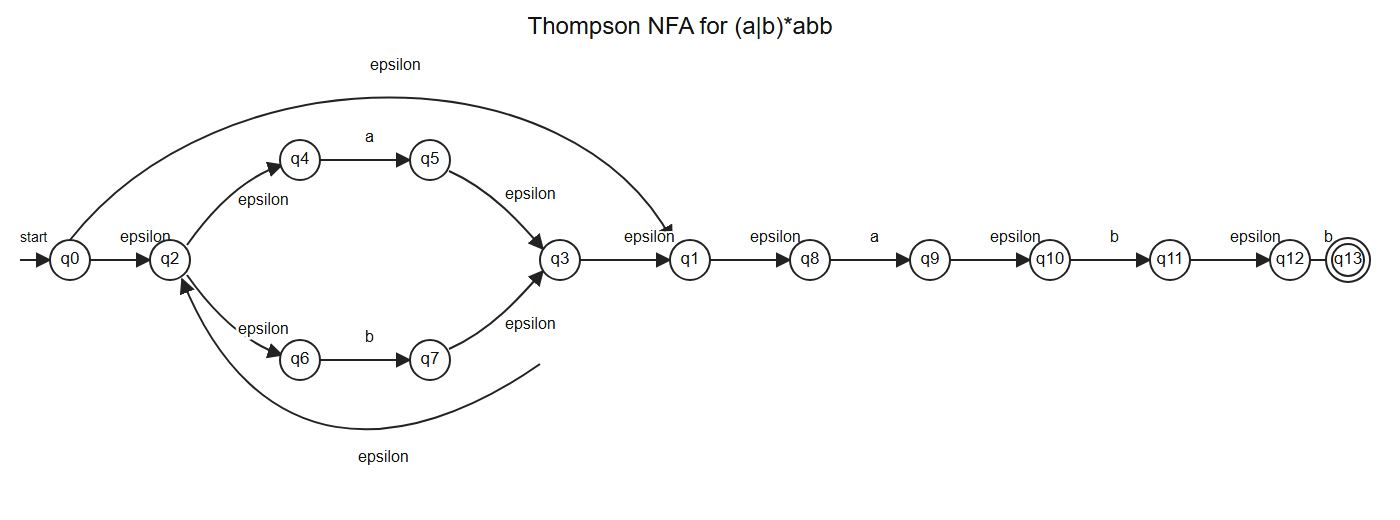
\includegraphics[width=0.82\linewidth]{figures/nfa-thompson-abstar-abb.png}
\par{\small Thompson NFA for (a|b)*abb}
\end{figure}

\begin{figure}[H]\centering
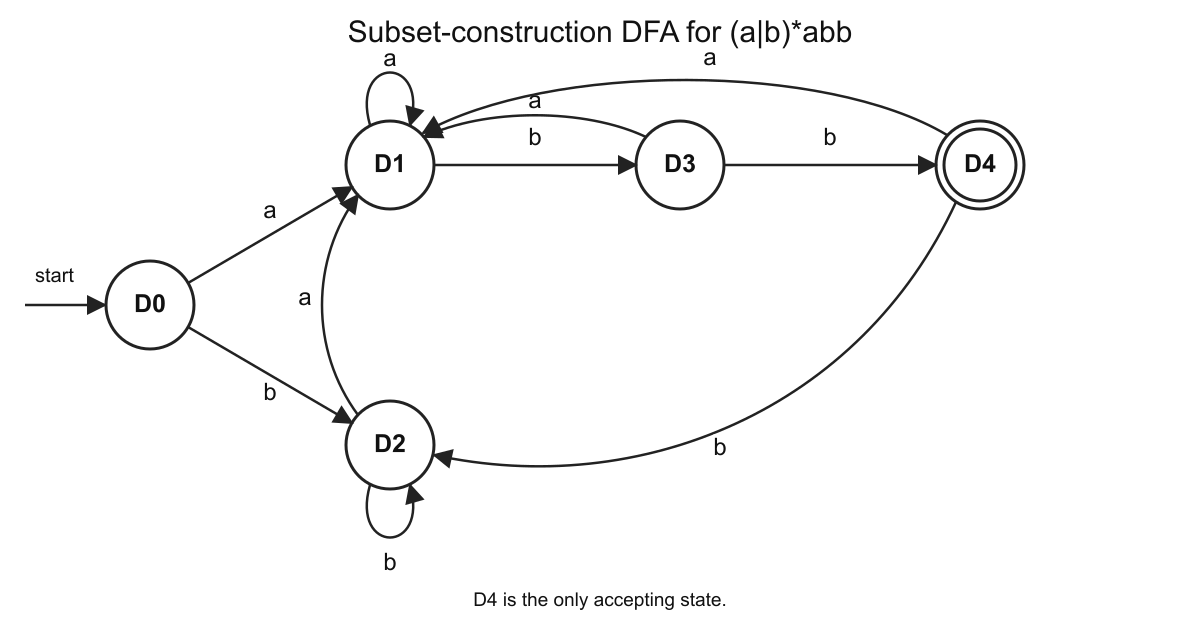
\includegraphics[width=0.82\linewidth]{figures/dfa-subset-abstar-abb.png}
\par{\small 子集构造 DFA for (a|b)*abb}
\end{figure}

\begin{figure}[H]\centering
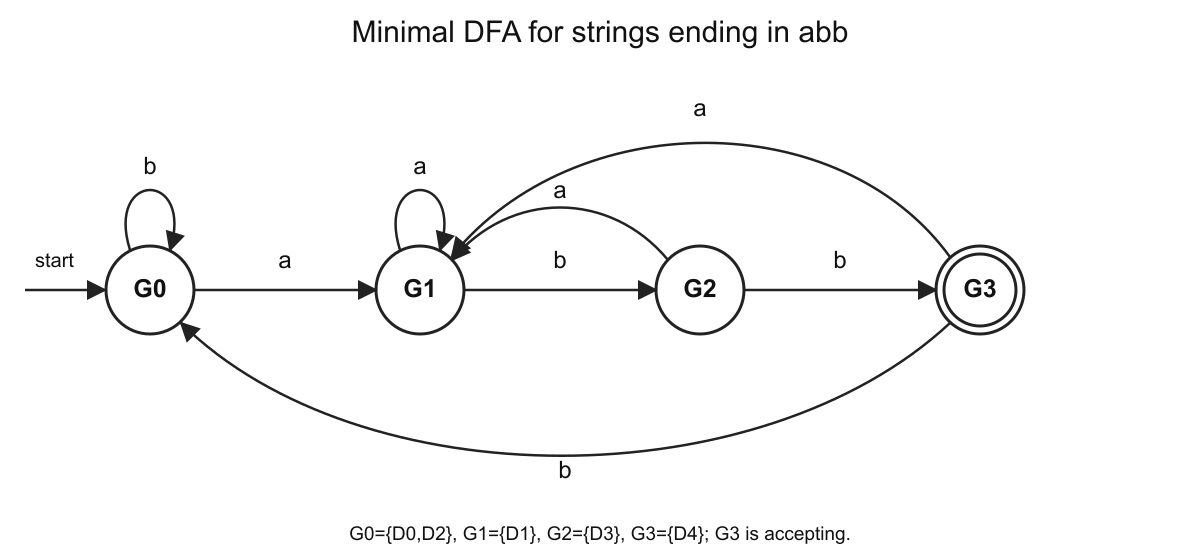
\includegraphics[width=0.82\linewidth]{figures/dfa-min-abstar-abb.png}
\par{\small 最小 DFA for (a|b)*abb}
\end{figure}

\paragraph*{1. Thompson NFA}

先把正则表达式拆成两部分：

\begin{Verbatim}[fontsize=\small,breaklines=true]
(a|b)* abb
\end{Verbatim}

\texttt{a|b} 用并联结构，\texttt{*} 在并联结构外加新入口和新出口，后面再顺序连接 \texttt{a}、\texttt{b}、\texttt{b}。按图中编号，可写为下面的 NFA 边表：

\begin{longtable}{|p{0.19\linewidth}|p{0.19\linewidth}|p{0.19\linewidth}|p{0.19\linewidth}|p{0.19\linewidth}|}
\hline
起点 & 边标号 & 终点 & 含义 &  \\
\hline
\endfirsthead
起点 & 边标号 & 终点 & 含义 &  \\
\hline
\endhead
q0 & epsilon & q2 & 进入 `(a & b)*` 的循环体 \\
\hline
q0 & epsilon & q1 & \texttt{*} 允许重复 0 次 &  \\
\hline
q2 & epsilon & q4 & 选择 \texttt{a} 分支 &  \\
\hline
q2 & epsilon & q6 & 选择 \texttt{b} 分支 &  \\
\hline
q4 & a & q5 & 匹配分支 \texttt{a} &  \\
\hline
q6 & b & q7 & 匹配分支 \texttt{b} &  \\
\hline
q5 & epsilon & q3 & \texttt{a} 分支结束 &  \\
\hline
q7 & epsilon & q3 & \texttt{b} 分支结束 &  \\
\hline
q3 & epsilon & q2 & \texttt{*} 回到循环入口 &  \\
\hline
q3 & epsilon & q1 & \texttt{*} 退出循环 &  \\
\hline
q1 & epsilon & q8 & 连接后缀 \texttt{abb} &  \\
\hline
q8 & a & q9 & 匹配后缀第 1 个字符 \texttt{a} &  \\
\hline
q9 & epsilon & q10 & 连接 &  \\
\hline
q10 & b & q11 & 匹配后缀第 2 个字符 \texttt{b} &  \\
\hline
q11 & epsilon & q12 & 连接 &  \\
\hline
q12 & b & q13 & 匹配后缀第 3 个字符 \texttt{b} &  \\
\hline
\end{longtable}

起始状态是 \texttt{q0}，接受状态是 \texttt{q13}。

\paragraph*{2. 子集构造 DFA}

从初始状态的 epsilon-closure 开始：

\begin{Verbatim}[fontsize=\small,breaklines=true]
D0 = epsilon-closure({q0}) = {q0,q1,q2,q4,q6,q8}
\end{Verbatim}

对每个 DFA 状态分别计算 \texttt{move(状态集合, 输入符号)}，再取 epsilon-closure，得到：

\begin{longtable}{|p{0.19\linewidth}|p{0.19\linewidth}|p{0.19\linewidth}|p{0.19\linewidth}|p{0.19\linewidth}|}
\hline
DFA 状态 & NFA 状态集合 & 输入 a 后 & 输入 b 后 & 是否接受 \\
\hline
\endfirsthead
DFA 状态 & NFA 状态集合 & 输入 a 后 & 输入 b 后 & 是否接受 \\
\hline
\endhead
D0 & \texttt{\textbackslash{}\{q0,q1,q2,q4,q6,q8\textbackslash{}\}} & D1 & D2 & 否 \\
\hline
D1 & \texttt{\textbackslash{}\{q1,q2,q3,q4,q5,q6,q8,q9,q10\textbackslash{}\}} & D1 & D3 & 否 \\
\hline
D2 & \texttt{\textbackslash{}\{q1,q2,q3,q4,q6,q7,q8\textbackslash{}\}} & D1 & D2 & 否 \\
\hline
D3 & \texttt{\textbackslash{}\{q1,q2,q3,q4,q6,q7,q8,q11,q12\textbackslash{}\}} & D1 & D4 & 否 \\
\hline
D4 & \texttt{\textbackslash{}\{q1,q2,q3,q4,q6,q7,q8,q13\textbackslash{}\}} & D1 & D2 & 是 \\
\hline
\end{longtable}

接受状态的判断依据是：DFA 状态集合中包含 NFA 接受状态 \texttt{q13}。因此只有 \texttt{D4} 是接受状态。

\paragraph*{3. DFA 最小化}

初始按接受状态和非接受状态分组：

\begin{Verbatim}[fontsize=\small,breaklines=true]
P0 = { {D4}, {D0,D1,D2,D3} }
\end{Verbatim}

继续比较非接受状态在输入 \texttt{a}、\texttt{b} 上到达的分组：

\begin{longtable}{|p{0.23\linewidth}|p{0.23\linewidth}|p{0.23\linewidth}|p{0.23\linewidth}|}
\hline
状态 & a 转移 & b 转移 & 区分依据 \\
\hline
\endfirsthead
状态 & a 转移 & b 转移 & 区分依据 \\
\hline
\endhead
D0 & D1 & D2 & \texttt{b} 不到接受组 \\
\hline
D1 & D1 & D3 & 与 D3 同型 \\
\hline
D2 & D1 & D2 & 与 D0 同型 \\
\hline
D3 & D1 & D4 & \texttt{b} 到接受组 \\
\hline
\end{longtable}

第一轮可以把 \texttt{D3} 与 \texttt{D0,D1,D2} 区分，因为 \texttt{D3} 在输入 \texttt{b} 后到达接受状态 \texttt{D4}。继续比较：

\begin{longtable}{|p{0.23\linewidth}|p{0.23\linewidth}|p{0.23\linewidth}|p{0.23\linewidth}|}
\hline
比较 & 输入 a & 输入 b & 结论 \\
\hline
\endfirsthead
比较 & 输入 a & 输入 b & 结论 \\
\hline
\endhead
D0 与 D2 & 都到 D1 & 都到 D2 & 等价，可合并 \\
\hline
D1 与 D0/D2 & \texttt{a} 到 D1 & \texttt{b} 到 D3，与 D0/D2 不同 & 不等价 \\
\hline
\end{longtable}

最终最小化分组为：

\begin{Verbatim}[fontsize=\small,breaklines=true]
G0 = {D0,D2}
G1 = {D1}
G2 = {D3}
G3 = {D4}
\end{Verbatim}

最小 DFA 转移表：

\begin{longtable}{|p{0.19\linewidth}|p{0.19\linewidth}|p{0.19\linewidth}|p{0.19\linewidth}|p{0.19\linewidth}|}
\hline
最小状态 & 原 DFA 状态 & 输入 a & 输入 b & 说明 \\
\hline
\endfirsthead
最小状态 & 原 DFA 状态 & 输入 a & 输入 b & 说明 \\
\hline
\endhead
G0 & \texttt{\textbackslash{}\{D0,D2\textbackslash{}\}} & G1 & G0 & 初态 \\
\hline
G1 & \texttt{\textbackslash{}\{D1\textbackslash{}\}} & G1 & G2 & 已匹配后缀前缀 \texttt{a} \\
\hline
G2 & \texttt{\textbackslash{}\{D3\textbackslash{}\}} & G1 & G3 & 已匹配后缀前缀 \texttt{ab} \\
\hline
G3 & \texttt{\textbackslash{}\{D4\textbackslash{}\}} & G1 & G0 & 终态，已匹配 \texttt{abb} \\
\hline
\end{longtable}

因此最小 DFA 的初态是 \texttt{G0}，终态是 \texttt{G3}。

\subsubsection*{二、LL(1) 分析答案}

\paragraph*{1. 消除直接左递归}

原文法中 \texttt{E -> E + T | T} 和 \texttt{T -> T * F | F} 都是直接左递归。套用规则：

\begin{Verbatim}[fontsize=\small,breaklines=true]
A  -> A alpha | beta
A  -> beta A'
A' -> alpha A' | epsilon
\end{Verbatim}

对 \texttt{E} 有 \texttt{alpha = + T}，\texttt{beta = T}；对 \texttt{T} 有 \texttt{alpha = * F}，\texttt{beta = F}。得到：

\begin{Verbatim}[fontsize=\small,breaklines=true]
E  -> T E'
E' -> + T E' | epsilon
T  -> F T'
T' -> * F T' | epsilon
F  -> ( E ) | id
\end{Verbatim}

\paragraph*{2. FIRST 集}

\begin{longtable}{|p{0.23\linewidth}|p{0.23\linewidth}|p{0.23\linewidth}|p{0.23\linewidth}|}
\hline
符号 & 推导依据 & FIRST 集 &  \\
\hline
\endfirsthead
符号 & 推导依据 & FIRST 集 &  \\
\hline
\endhead
F & `F -> ( E ) & id` & \texttt{\textbackslash{}\{ (, id \textbackslash{}\}} \\
\hline
T' & `T' -> * F T' & epsilon` & \texttt{\textbackslash{}\{ *, epsilon \textbackslash{}\}} \\
\hline
T & \texttt{T -> F T'}，F 不能推出 epsilon & \texttt{\textbackslash{}\{ (, id \textbackslash{}\}} &  \\
\hline
E' & `E' -> + T E' & epsilon` & \texttt{\textbackslash{}\{ +, epsilon \textbackslash{}\}} \\
\hline
E & \texttt{E -> T E'}，T 不能推出 epsilon & \texttt{\textbackslash{}\{ (, id \textbackslash{}\}} &  \\
\hline
\end{longtable}

\paragraph*{3. FOLLOW 集}

先放入开始符号的结束标记：

\begin{Verbatim}[fontsize=\small,breaklines=true]
FOLLOW(E) = { $ }
\end{Verbatim}

再逐条产生式传播：

\begin{longtable}{|p{0.31\linewidth}|p{0.31\linewidth}|p{0.31\linewidth}|}
\hline
产生式位置 & 推导规则 & 新增内容 \\
\hline
\endfirsthead
产生式位置 & 推导规则 & 新增内容 \\
\hline
\endhead
\texttt{F -> ( E )} & E 后面是 \texttt{)} & \texttt{)} 加入 FOLLOW(E) \\
\hline
\texttt{E -> T E'} & T 后面是 E'，加入 FIRST(E') 去掉 epsilon & \texttt{+} 加入 FOLLOW(T) \\
\hline
\texttt{E -> T E'} & E' 在末尾，加入 FOLLOW(E) & \texttt{)}、\texttt{\textbackslash{}\$} 加入 FOLLOW(E') \\
\hline
\texttt{E -> T E'} & E' 可推出 epsilon，FOLLOW(E) 加入 FOLLOW(T) & \texttt{)}、\texttt{\textbackslash{}\$} 加入 FOLLOW(T) \\
\hline
\texttt{E' -> + T E'} & T 后面是 E'，加入 FIRST(E') 去掉 epsilon & \texttt{+} 加入 FOLLOW(T) \\
\hline
\texttt{E' -> + T E'} & E' 在末尾，加入 FOLLOW(E') & \texttt{)}、\texttt{\textbackslash{}\$} 保持在 FOLLOW(E') \\
\hline
\texttt{T -> F T'} & F 后面是 T'，加入 FIRST(T') 去掉 epsilon & \texttt{*} 加入 FOLLOW(F) \\
\hline
\texttt{T -> F T'} & T' 可推出 epsilon，FOLLOW(T) 加入 FOLLOW(F) & \texttt{+}、\texttt{)}、\texttt{\textbackslash{}\$} 加入 FOLLOW(F) \\
\hline
\texttt{T -> F T'} & T' 在末尾，加入 FOLLOW(T) & \texttt{+}、\texttt{)}、\texttt{\textbackslash{}\$} 加入 FOLLOW(T') \\
\hline
\end{longtable}

最终：

\begin{longtable}{|p{0.47\linewidth}|p{0.47\linewidth}|}
\hline
非终结符 & FOLLOW 集 \\
\hline
\endfirsthead
非终结符 & FOLLOW 集 \\
\hline
\endhead
E & \texttt{\textbackslash{}\{ ), \textbackslash{}\$ \textbackslash{}\}} \\
\hline
E' & \texttt{\textbackslash{}\{ ), \textbackslash{}\$ \textbackslash{}\}} \\
\hline
T & \texttt{\textbackslash{}\{ +, ), \textbackslash{}\$ \textbackslash{}\}} \\
\hline
T' & \texttt{\textbackslash{}\{ +, ), \textbackslash{}\$ \textbackslash{}\}} \\
\hline
F & \texttt{\textbackslash{}\{ *, +, ), \textbackslash{}\$ \textbackslash{}\}} \\
\hline
\end{longtable}

\paragraph*{4. 预测分析表}

填表规则：对 \texttt{A -> alpha}，把产生式填入 \texttt{FIRST(alpha)} 中的终结符列；若 \texttt{alpha} 可推出 epsilon，则填入 \texttt{FOLLOW(A)} 中的列。

\begin{longtable}{|p{0.31\linewidth}|p{0.31\linewidth}|p{0.31\linewidth}|}
\hline
产生式 & 填表依据 & 填入表项 \\
\hline
\endfirsthead
产生式 & 填表依据 & 填入表项 \\
\hline
\endhead
\texttt{E -> T E'} & \texttt{FIRST(T E')=\textbackslash{}\{ (, id \textbackslash{}\}} & \texttt{M[E,(]}，\texttt{M[E,id]} \\
\hline
\texttt{E' -> + T E'} & \texttt{FIRST(+ T E')=\textbackslash{}\{ + \textbackslash{}\}} & \texttt{M[E',+]} \\
\hline
\texttt{E' -> epsilon} & \texttt{FOLLOW(E')=\textbackslash{}\{ ), \textbackslash{}\$ \textbackslash{}\}} & \texttt{M[E',)]}，\texttt{M[E',\textbackslash{}\$]} \\
\hline
\texttt{T -> F T'} & \texttt{FIRST(F T')=\textbackslash{}\{ (, id \textbackslash{}\}} & \texttt{M[T,(]}，\texttt{M[T,id]} \\
\hline
\texttt{T' -> * F T'} & \texttt{FIRST(* F T')=\textbackslash{}\{ * \textbackslash{}\}} & \texttt{M[T',*]} \\
\hline
\texttt{T' -> epsilon} & \texttt{FOLLOW(T')=\textbackslash{}\{ +, ), \textbackslash{}\$ \textbackslash{}\}} & \texttt{M[T',+]}，\texttt{M[T',)]}，\texttt{M[T',\textbackslash{}\$]} \\
\hline
\texttt{F -> ( E )} & \texttt{FIRST(( E ))=\textbackslash{}\{ ( \textbackslash{}\}} & \texttt{M[F,(]} \\
\hline
\texttt{F -> id} & \texttt{FIRST(id)=\textbackslash{}\{ id \textbackslash{}\}} & \texttt{M[F,id]} \\
\hline
\end{longtable}

完整预测分析表如下，空白处为 error：

\begin{longtable}{|p{0.13\linewidth}|p{0.13\linewidth}|p{0.13\linewidth}|p{0.13\linewidth}|p{0.13\linewidth}|p{0.13\linewidth}|p{0.13\linewidth}|}
\hline
非终结符 & \texttt{(} & \texttt{id} & \texttt{+} & \texttt{*} & \texttt{)} & \texttt{\textbackslash{}\$} \\
\hline
\endfirsthead
非终结符 & \texttt{(} & \texttt{id} & \texttt{+} & \texttt{*} & \texttt{)} & \texttt{\textbackslash{}\$} \\
\hline
\endhead
E & \texttt{E -> T E'} & \texttt{E -> T E'} & error & error & error & error \\
\hline
E' & error & error & \texttt{E' -> + T E'} & error & \texttt{E' -> epsilon} & \texttt{E' -> epsilon} \\
\hline
T & \texttt{T -> F T'} & \texttt{T -> F T'} & error & error & error & error \\
\hline
T' & error & error & \texttt{T' -> epsilon} & \texttt{T' -> * F T'} & \texttt{T' -> epsilon} & \texttt{T' -> epsilon} \\
\hline
F & \texttt{F -> ( E )} & \texttt{F -> id} & error & error & error & error \\
\hline
\end{longtable}

每个表项最多一条产生式，因此消除左递归后的文法是 LL(1) 文法。

\subsubsection*{三、LR(0) 项集族与 SLR 分析表答案}

\paragraph*{1. 规范 LR(0) 项集族}

增广文法为：

\begin{Verbatim}[fontsize=\small,breaklines=true]
S' -> S
S  -> C C
C  -> c C | d
\end{Verbatim}

从 \texttt{I0 = closure(\textbackslash{}\{S' -> . S\textbackslash{}\})} 开始：

\begin{Verbatim}[fontsize=\small,breaklines=true]
I0:
S' -> . S
S  -> . C C
C  -> . c C
C  -> . d

I1 = GOTO(I0, S):
S' -> S .

I2 = GOTO(I0, C):
S -> C . C
C -> . c C
C -> . d

I3 = GOTO(I0, c):
C -> c . C
C -> . c C
C -> . d

I4 = GOTO(I0, d):
C -> d .

I5 = GOTO(I2, C):
S -> C C .

I6 = GOTO(I3, C):
C -> c C .
\end{Verbatim}

其中 \texttt{GOTO(I3,c)=I3}，因为 \texttt{C -> c . C} 移过 \texttt{c} 后再次得到 \texttt{C -> c . C} 并闭包出同样项目。

\paragraph*{2. GOTO 转移}

\begin{longtable}{|p{0.31\linewidth}|p{0.31\linewidth}|p{0.31\linewidth}|}
\hline
来源状态 & 文法符号 & 目标状态 \\
\hline
\endfirsthead
来源状态 & 文法符号 & 目标状态 \\
\hline
\endhead
I0 & S & I1 \\
\hline
I0 & C & I2 \\
\hline
I0 & c & I3 \\
\hline
I0 & d & I4 \\
\hline
I2 & C & I5 \\
\hline
I2 & c & I3 \\
\hline
I2 & d & I4 \\
\hline
I3 & C & I6 \\
\hline
I3 & c & I3 \\
\hline
I3 & d & I4 \\
\hline
\end{longtable}

\paragraph*{3. FOLLOW 集}

\begin{longtable}{|p{0.31\linewidth}|p{0.31\linewidth}|p{0.31\linewidth}|}
\hline
非终结符 & 推导依据 & FOLLOW \\
\hline
\endfirsthead
非终结符 & 推导依据 & FOLLOW \\
\hline
\endhead
S & S 是开始符号 & \texttt{\textbackslash{}\{ \textbackslash{}\$ \textbackslash{}\}} \\
\hline
C & \texttt{S -> C C} 中第一个 C 后面是 C，加入 FIRST(C)=\{c,d\}；第二个 C 在末尾，加入 FOLLOW(S) & \texttt{\textbackslash{}\{ c, d, \textbackslash{}\$ \textbackslash{}\}} \\
\hline
\end{longtable}

\paragraph*{4. SLR ACTION/GOTO 表}

填表规则：

\begin{Verbatim}[fontsize=\small,breaklines=true]
A -> alpha . a beta 形成移进项，ACTION[state,a] = shift。
A -> alpha . 且 A 不是 S' 时，在 FOLLOW(A) 上填 reduce。
S' -> S . 时，在 $ 上填 accept。
\end{Verbatim}

逐状态填表：

\begin{longtable}{|p{0.31\linewidth}|p{0.31\linewidth}|p{0.31\linewidth}|}
\hline
状态 & 项目依据 & 表项 \\
\hline
\endfirsthead
状态 & 项目依据 & 表项 \\
\hline
\endhead
0 & \texttt{C -> . c C}，\texttt{C -> . d}，\texttt{S -> . C C}，\texttt{S' -> . S} & \texttt{ACTION[0,c]=s3}，\texttt{ACTION[0,d]=s4}，\texttt{GOTO[0,C]=2}，\texttt{GOTO[0,S]=1} \\
\hline
1 & \texttt{S' -> S .} & \texttt{ACTION[1,\textbackslash{}\$]=acc} \\
\hline
2 & \texttt{C -> . c C}，\texttt{C -> . d}，\texttt{S -> C . C} & \texttt{ACTION[2,c]=s3}，\texttt{ACTION[2,d]=s4}，\texttt{GOTO[2,C]=5} \\
\hline
3 & \texttt{C -> . c C}，\texttt{C -> . d}，\texttt{C -> c . C} & \texttt{ACTION[3,c]=s3}，\texttt{ACTION[3,d]=s4}，\texttt{GOTO[3,C]=6} \\
\hline
4 & \texttt{C -> d .} & 在 FOLLOW(C)=\{c,d,\$\} 上填 \texttt{r(C -> d)} \\
\hline
5 & \texttt{S -> C C .} & 在 FOLLOW(S)=\{\$\} 上填 \texttt{r(S -> C C)} \\
\hline
6 & \texttt{C -> c C .} & 在 FOLLOW(C)=\{c,d,\$\} 上填 \texttt{r(C -> c C)} \\
\hline
\end{longtable}

完整表：

\begin{longtable}{|p{0.16\linewidth}|p{0.16\linewidth}|p{0.16\linewidth}|p{0.16\linewidth}|p{0.16\linewidth}|p{0.16\linewidth}|}
\hline
状态 & ACTION c & ACTION d & ACTION \$ & GOTO S & GOTO C \\
\hline
\endfirsthead
状态 & ACTION c & ACTION d & ACTION \$ & GOTO S & GOTO C \\
\hline
\endhead
0 & s3 & s4 & error & 1 & 2 \\
\hline
1 & error & error & acc & error & error \\
\hline
2 & s3 & s4 & error & error & 5 \\
\hline
3 & s3 & s4 & error & error & 6 \\
\hline
4 & r(C -> d) & r(C -> d) & r(C -> d) & error & error \\
\hline
5 & error & error & r(S -> C C) & error & error \\
\hline
6 & r(C -> c C) & r(C -> c C) & r(C -> c C) & error & error \\
\hline
\end{longtable}

\subsubsection*{四、语义分析答案}

\paragraph*{1. 声明文法的 L 属性 SDD}

题目要求每个 \texttt{id} 都记录从 \texttt{T} 得到的类型。类型信息从左边的 \texttt{T} 传给右边的 \texttt{L}，所以需要继承属性。

\begin{longtable}{|p{0.47\linewidth}|p{0.47\linewidth}|}
\hline
产生式 & 语义规则或动作 \\
\hline
\endfirsthead
产生式 & 语义规则或动作 \\
\hline
\endhead
\texttt{D -> T L} & \texttt{L.in = T.type} \\
\hline
\texttt{T -> int} & \texttt{T.type = int} \\
\hline
\texttt{T -> float} & \texttt{T.type = float} \\
\hline
\texttt{L -> id L'} & \texttt{addType(id.name, L.in)}；\texttt{L'.in = L.in} \\
\hline
\texttt{L' -> , id L'1} & \texttt{addType(id.name, L'.in)}；\texttt{L'1.in = L'.in} \\
\hline
\texttt{L' -> epsilon} & 不需要插入新标识符 \\
\hline
\end{longtable}

它是 L 属性定义的原因：

\begin{Verbatim}[fontsize=\small,breaklines=true]
L.in 只依赖父结点 D 中左侧兄弟 T.type。
L'.in 只依赖父结点 L 或 L' 的继承属性。
没有任何继承属性依赖右侧兄弟结点。
\end{Verbatim}

如果输入是 \texttt{float x, y}，执行顺序是：

\begin{longtable}{|p{0.31\linewidth}|p{0.31\linewidth}|p{0.31\linewidth}|}
\hline
步骤 & 动作 & 符号表效果 \\
\hline
\endfirsthead
步骤 & 动作 & 符号表效果 \\
\hline
\endhead
1 & \texttt{T -> float} & \texttt{T.type=float} \\
\hline
2 & \texttt{D -> T L} & \texttt{L.in=float} \\
\hline
3 & 识别 \texttt{x} & 插入 \texttt{x : float} \\
\hline
4 & 识别 \texttt{y} & 插入 \texttt{y : float} \\
\hline
\end{longtable}

\paragraph*{2. 后缀表达式的 S 属性 SDD}

题目要求 \texttt{code} 表示后缀表达式，只需要综合属性：

\begin{longtable}{|p{0.16\linewidth}|p{0.16\linewidth}|p{0.16\linewidth}|p{0.16\linewidth}|p{0.16\linewidth}|p{0.16\linewidth}|}
\hline
产生式 & 语义规则 &  &  &  &  \\
\hline
\endfirsthead
产生式 & 语义规则 &  &  &  &  \\
\hline
\endhead
\texttt{E -> E1 + T} & `E.code = E1.code &  & T.code &  & "+"` \\
\hline
\texttt{E -> T} & \texttt{E.code = T.code} &  &  &  &  \\
\hline
\texttt{T -> num} & \texttt{T.code = num.lexeme} &  &  &  &  \\
\hline
\end{longtable}

对 \texttt{3 + 4 + 5}，原文法左递归，表达式按左结合分析为 \texttt{((3 + 4) + 5)}：

\begin{longtable}{|p{0.47\linewidth}|p{0.47\linewidth}|}
\hline
子表达式 & 后缀 code \\
\hline
\endfirsthead
子表达式 & 后缀 code \\
\hline
\endhead
\texttt{3} & \texttt{3} \\
\hline
\texttt{4} & \texttt{4} \\
\hline
\texttt{3 + 4} & \texttt{3 4 +} \\
\hline
\texttt{5} & \texttt{5} \\
\hline
\texttt{(3 + 4) + 5} & \texttt{3 4 + 5 +} \\
\hline
\end{longtable}

最终：

\begin{Verbatim}[fontsize=\small,breaklines=true]
E.code = 3 4 + 5 +
\end{Verbatim}

\subsubsection*{五、中间代码答案}

\paragraph*{1. 短路求值与回填}

布尔表达式是：

\begin{Verbatim}[fontsize=\small,breaklines=true]
((x < y) && (y < z)) || (x == z)
\end{Verbatim}

先看优先级：\texttt{\textbackslash{}\&\textbackslash{}\&} 高于 \texttt{||}，因此先求 \texttt{(x < y) \textbackslash{}\&\textbackslash{}\& (y < z)}；如果左侧 \texttt{\textbackslash{}\&\textbackslash{}\&} 整体为真，则整个 \texttt{||} 为真，不再求 \texttt{x == z}；如果左侧 \texttt{\textbackslash{}\&\textbackslash{}\&} 为假，才去求 \texttt{x == z}。

回填思路如下：

\begin{longtable}{|p{0.31\linewidth}|p{0.31\linewidth}|p{0.31\linewidth}|}
\hline
判断 & 真出口 & 假出口 \\
\hline
\endfirsthead
判断 & 真出口 & 假出口 \\
\hline
\endhead
\texttt{x < y} & 继续判断 \texttt{y < z} & 去判断 \texttt{x == z} \\
\hline
\texttt{y < z} & then 分支 & 去判断 \texttt{x == z} \\
\hline
\texttt{x == z} & then 分支 & else 分支 \\
\hline
\end{longtable}

回填后的三地址码：

\begin{Verbatim}[fontsize=\small,breaklines=true]
1: if x < y goto 3
2: goto 5
3: if y < z goto 7
4: goto 5
5: if x == z goto 7
6: goto 9
7: a = 2
8: goto 10
9: a = 3
10:
\end{Verbatim}

逐行检查：

\begin{longtable}{|p{0.23\linewidth}|p{0.23\linewidth}|p{0.23\linewidth}|p{0.23\linewidth}|}
\hline
行号 & 作用 &  &  \\
\hline
\endfirsthead
行号 & 作用 &  &  \\
\hline
\endhead
1-2 & 判断 \texttt{x < y}，假时短路到 ` &  & ` 的右操作数 \\
\hline
3-4 & 判断 \texttt{y < z}，假时继续判断 \texttt{x == z} &  &  \\
\hline
5-6 & 判断 \texttt{x == z}，真到 then，假到 else &  &  \\
\hline
7-10 & then/else 赋值并汇合 &  &  \\
\hline
\end{longtable}

\paragraph*{2. 循环 SSA}

循环变量 \texttt{i} 和 \texttt{s} 都在循环前有初值，又在循环体中被重新定义，因此循环头需要两个 phi 函数。

\begin{longtable}{|p{0.23\linewidth}|p{0.23\linewidth}|p{0.23\linewidth}|p{0.23\linewidth}|}
\hline
变量 & 循环前定义 & 循环体回边定义 & 循环头版本 \\
\hline
\endfirsthead
变量 & 循环前定义 & 循环体回边定义 & 循环头版本 \\
\hline
\endhead
i & \texttt{i1 = 0} & \texttt{i3 = i2 + 1} & \texttt{i2 = phi(i1, i3)} \\
\hline
s & \texttt{s1 = 0} & \texttt{s3 = s2 + i2} & \texttt{s2 = phi(s1, s3)} \\
\hline
\end{longtable}

SSA 风格三地址码：

\begin{Verbatim}[fontsize=\small,breaklines=true]
entry:
i1 = 0
s1 = 0
goto L_header

L_header:
i2 = phi(i1, i3)
s2 = phi(s1, s3)
t1 = i2 < n
if t1 goto L_body else L_exit

L_body:
s3 = s2 + i2
i3 = i2 + 1
goto L_header

L_exit:
\end{Verbatim}

phi 的位置在循环头 \texttt{L\textbackslash{}\_header}，原因是控制流有两条路径到达循环头：一次来自 \texttt{entry}，另一次来自循环体回边。
\end{document}
